\documentclass[10pt,twocolumn]{article}
\usepackage[margin=0.6in,top=0.55in,bottom=0.55in]{geometry}
\usepackage{amsmath,amssymb}
\usepackage{booktabs}
\usepackage{graphicx}
\usepackage[font=small,skip=3pt]{caption}
\usepackage{hyperref}
\usepackage{enumitem}
\usepackage{microtype}
\usepackage{titlesec}
\usepackage{url}
\usepackage{setspace}
\setstretch{0.9}

\titlespacing*{\section}{0pt}{4pt}{1.5pt}
\titlespacing*{\subsection}{0pt}{2.5pt}{0.5pt}
\titlespacing*{\paragraph}{0pt}{2pt}{0.6em}
\renewcommand{\arraystretch}{0.9}
\setlength{\columnsep}{14pt}
\setlength{\belowcaptionskip}{0pt}
\setlength{\textfloatsep}{6pt}
\setlength{\intextsep}{6pt}
\setlength{\parskip}{0pt}
\abovedisplayskip=4pt \belowdisplayskip=4pt
\abovedisplayshortskip=2pt \belowdisplayshortskip=2pt
\raggedbottom

\hypersetup{colorlinks=true,linkcolor=blue,urlcolor=blue,citecolor=blue,
  pdftitle={Knee MRI Abnormality Detection with LLM-Read Report Labels},
  pdfauthor={Abdul Samad Zaheer Khan}}

\begin{document}
\twocolumn[{%
\begin{center}
\vspace*{0.4em}
{\Large\textbf{Knee MRI Abnormality Detection with LLM-Read Report Labels:\\
Approaches and Validation Lessons from the RSNA Kaggle Challenge}\par}
\vspace{0.9em}
{\normalsize Abdul Samad Zaheer Khan \quad
\small New York University \quad
\small\texttt{ak9943@nyu.edu} \quad
\small\url{https://github.com/abdulllkhan/RSNA}\\[2pt]
\small November 2026\par}
\vspace{0.7em}
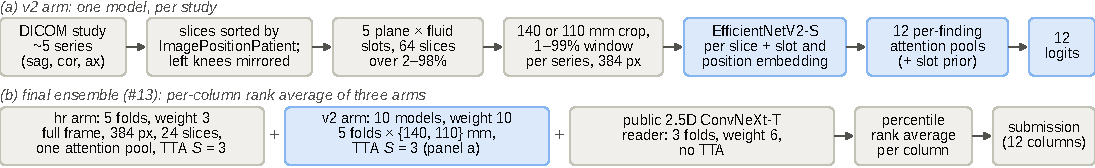
\includegraphics[width=\textwidth]{figures/pipeline.pdf}
\captionsetup{hypcap=false}
\captionof{figure}{Pipeline. (a)~One v2 model: anatomically ordered, laterality-canonical slices in five
plane\,$\times$\,fluid slots; a shared EfficientNetV2-S; 12 per-finding attention pools. (b)~Submission:
per-column percentile-rank average of three arms (3\,:\,10\,:\,6).}
\label{fig:pipeline}
\end{center}
\vspace{0.2em}
}]
\thispagestyle{empty}

%% ---------------------------------------------
\begin{abstract}
\noindent
We describe our entry to the RSNA Knee Abnormality Detection challenge on Kaggle: 12 findings per knee MRI study,
scored by macro ROC AUC, with radiologist labels for only 58 of 4,407 training studies. We trained on labels
that large language models (LLMs) extracted from the reports and rank-averaged 15 EfficientNetV2-S models with a
public 2.5D ConvNeXt-T reader, scoring \textbf{0.927 private} (0.941 public), rank 3,011 of 6,299: a mid-table result against a
top private score of 0.960. Model choices were gated on 5-fold out-of-fold (OOF) AUC and the 58 gold studies. Private ran 0.014--0.020
below public with our 15 submissions in the same order, and our first-choice final was our best private entry; the gap
to the top came from the approach, not from overfitting. Local gains transferred for our own models trained on report
labels, but not for distillation on OOF-derived targets or for a validated public model (+0.0069 OOF; +0.001 public,
+0.002 private).
\end{abstract}

%% ---------------------------------------------
\section{Task and data}

The challenge~\cite{rsna} asks for a probability of each of 12 findings per study (ACL, MCL, medial and lateral
meniscal tear, medial, lateral and patellofemoral osteoarthritis, effusion, synovitis, Baker's cyst, contusion,
fracture), scored by the mean of the 12 ROC AUCs, so only within-column ranks matter. The 4,407 training studies
(about five series each) have free-text reports in several languages but only 58 radiologist labels. The
$\approx$1,300 hidden test studies have images only and are predicted offline on one T4 GPU within 9\,h; public and
private scores use disjoint subsets.

%% ---------------------------------------------
\section{Labels from reports}

Targets come from public LLM-extracted report labels~\cite{labels}: first one soft table (stevenleehans v4; 0.893
AUC on gold), finally a soft consensus of three (stevenleehans v2, pilkwang v2, lixin73) with per-cell weight
$w=0.15+0.85\,(0.65\,a+0.35\,c)$ from teacher agreement $a$ and certainty $c$, plus the gold studies at $w=3$, as in
the public notebooks. Every table was leak-checked against gold first (one public merge reproduces all 58 labels). A
local Gemma-3-27B~\cite{gemma} re-read for synovitis lost on gold (0.722 vs.\ 0.790): 14 of its 27 gold positives
have reports that never mention the synovium.

%% ---------------------------------------------
\section{Models and ensemble}

\paragraph{v2 arm (Fig.~\ref{fig:pipeline}a).} Following pilkwang's public baseline and its descendants, each chosen
series is decoded once, centre-cropped to 140 or 110\,mm (from \texttt{PixelSpacing}), windowed at its own
1st--99th percentiles and resized to 384\,px. Slices are ordered by \texttt{ImagePositionPatient} (file order matched
anatomy in none of 400 sampled series) and fill five plane\,$\times$\,fluid slots (sagittal 18\,+\,14, coronal
12\,+\,8, axial 12) spaced over 2--98\% of the stack. Left knees are mirrored to a right-knee frame (side from the
DICOM tag or, when absent, image-centre geometry; 97.5\% agreement). An
EfficientNetV2-S~\cite{effnetv2} (timm~\cite{timm}) embeds each slice; with slot and position embeddings, 12
per-finding gated-attention pools~\cite{ilse} with a fixed anatomical slot prior ($+0.55$ logit) feed 12 linear
heads. Training: weighted soft binary cross-entropy, 38 slices per study (64 at test), AdamW at $3{\times}10^{-4}$ for all
layers, cosine schedule, EMA, 10 epochs (4.3--4.8\,h per fold on an NVIDIA GB10). Our first v2 run, with the
$0.1\times$ backbone rate ($2{\times}10^{-5}$) of the public ViT notebooks, scored 0.031 lower on fold 0.

\paragraph{hr arm.} An older high-resolution, full-frame arm (24 slices in file order, i.e.\ at effectively random positions;
per-slice min--max; one attention pool; stevenleehans v4 labels) is weak alone (0.871 on fold 0) but different.

\paragraph{Ensemble (Fig.~\ref{fig:pipeline}b).} Per-column percentile ranks are averaged with weights hr\,3,
v2\,10 (five 140\,mm and five 110\,mm fold models) and reader\,6 (Sec.~\ref{sec:reader}), set on a coarse grid on
stitched OOF; hr and v2 models also run on $S{=}3$ phase-shifted slice grids (slot-phase test-time augmentation, TTA). Series are decoded
once per crop; the hidden run takes about 5\,h.

%% ---------------------------------------------
\section{Validation protocol}

Each candidate gets (i)~stitched 5-fold OOF macro AUC on all 4,407 studies against the binarised stevenleehans v4
labels, each study scored by the model that did not train on it, and (ii)~AUC on the 58 gold studies, each scored by
the fold that held it out: one large but report-based, one true but with 9--35 positives per finding. Gates were
fixed in advance (e.g.\ a new member had to add $\geq{+0.003}$ OOF without lowering gold). Submissions needed about
$+0.005$ expected gain (the board shows three decimals) or served as a pre-registered calibration of a new kind of
member. Finals were picked by local validation under a decision table fixed in advance; nothing was fitted to the
board.

%% ---------------------------------------------
\section{Results}

\begin{figure}[t]
\centering
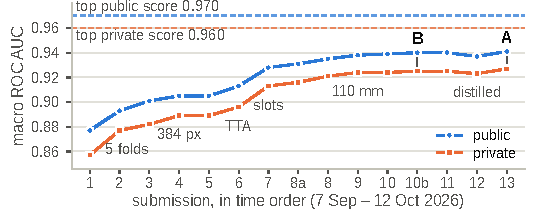
\includegraphics[width=\columnwidth]{figures/submissions.pdf}
\caption{All 15 submissions in time order (numbered as in our log). Notes name the change behind a step; A, B:
finals.}
\label{fig:subs}
\end{figure}

Figure~\ref{fig:subs} shows all submissions. The big steps were fold ensembling of the 224\,px baseline (+0.016 public, +0.020 private;
invisible to OOF, where each study is scored by one model), the 384\,px arm, TTA and above all the slot contract: one
fold-0 v2 model added +0.015/+0.017 and the full v2 arm reached 0.940/0.925 (\#10b). Private ran 0.014--0.020 below
public and no two submissions swapped order (ties aside; Kendall $\tau_b=0.995$). Final A (\#13, best local
validation) is also our best private score; B is \#10b (own models only). We rose from 3,163rd (public) to 3,011th
(private). For our own \mbox{v2-era} entries (\#8--\#10b),
public$-$OOF stayed at $+0.048$ to $+0.050$ and private$-$OOF at $+0.034$ to $+0.035$.

\begin{figure}[t]
\centering
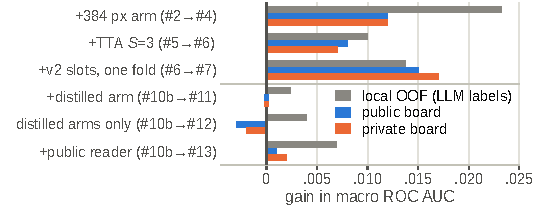
\includegraphics[width=\columnwidth]{figures/transfer.pdf}
\caption{Local vs.\ board gain of single changes (OOF on LLM labels; v2 row: fold 0 only; reader: 2,668
studies).}
\label{fig:transfer}
\end{figure}

In Figure~\ref{fig:transfer}, the first three changes transferred at 0.5--1.2$\times$ their OOF gain; the others
did not.
\emph{Distillation}, retraining v2 arms on targets mixed 50/50 from the consensus and the v2 arms' own OOF
predictions, raised OOF by up to $+0.0040$ (gold $+0.0074$) yet scored 0.000/$-0.003$ public and 0.000/$-0.002$
private: a student's targets carry information from models that saw its held-out fold, so both local anchors were
optimistic.

%% ---------------------------------------------
\section{Validating a public model}
\label{sec:reader}

goodpjw2008's reader~\cite{reader} (Apache-2.0; ConvNeXt-T~\cite{convnext} on slice triplets, a study-level
transformer, per-finding pools) has a recoverable split: its GroupKFold over report text re-derives from the
competition CSV and excludes gold. We ported its inference verbatim and proved the split: each checkpoint is
0.057--0.067 worse on its own re-derived fold than on its training folds, while a wrong split shows no gap. Its honest
OOF on 2,610 held-out studies is 0.8885 (gold 0.9105). At weight 6 (chosen on OOF from a pre-registered grid) it adds
$+0.0069$ OOF (95\% CI $+0.0058$ to $+0.0080$) and $+0.0023$ gold; a leaky three-checkpoint mean would have claimed $+0.0235$. The board
gave $+0.001$ public and $+0.002$ private (about 1/7 and 2/7 of that), though its Kaggle outputs matched ours to $3{\times}10^{-4}$: a recovered
split is necessary, not sufficient.

%% ---------------------------------------------
\section{Engineering lessons}

Four silent failures that would each have shipped an all-0.5 file were caught before submitting: a P100 that
Kaggle's PyTorch no longer supports (we pin the T4), bf16 convolutions on the T4 (fp16 instead), a JPEG-trained
pipeline meeting the DICOM test mount, and a fingerprint check aborting on cross-GPU drift. The
costliest bug was quiet: the 110\,mm checkpoints stored the default 140\,mm crop and the notebook used the first
member's crop for all, so in two submissions the 110\,mm arm saw 140\,mm crops ($-0.0106$ on fold 0); reading the
kernel log revealed it. The 9\,h limit capped the ensemble: 20--25 v2 models at $S{=}3$ would need 8.3--9\,h.

%% ---------------------------------------------
\section{Limits and next steps}

\begin{table}[t]
\centering\footnotesize
\setlength{\tabcolsep}{4pt}
\begin{tabular}{@{}lrl@{}}
\toprule
\textbf{Idea (closed)} & \textbf{$\Delta$AUC} & \textbf{Measured on} \\
\midrule
512\,px at the 110\,mm crop & $-0.0031$ & fold-0 model \\
2.5D context ($j\pm1$ as channels) & $0.0000$ & fold-0 model \\
170\,mm crop as a 4th arm & $+0.0004$ & fold-0 ensemble \\
CoAtNet-2, public recipe & $+0.0003$ & fold-0 ensemble \\
Second seed of both v2 arms & $+0.0005$ & final ensemble \\
TTA $S{=}5$ instead of 3 & $+0.0001$ & stitched ensemble \\
Cross-crop TTA & $\leq{+0.0002}$ & fold-0 ensemble \\
Per-column arm weights & $+0.0004$ & nested 5-fold \\
Protocol features (series counts) & $+0.0002$ & stitched ensemble \\
Distillation (Fig.~\ref{fig:transfer}) & $+0.0040$ & stitched ensemble \\
\bottomrule
\end{tabular}
\caption{Closed ideas ($\Delta$ OOF AUC on LLM labels); CoAtNet-2 and protocol features also cost gold ($-0.0017$,
$-0.0013$).}
\label{tab:neg}
\end{table}

Table~\ref{tab:neg} lists closed ideas: with the slot contract in place the ensemble saturated near 0.890 OOF, and
CoAtNet-2~\cite{coatnet}, trained with dreaddevelopment's public ``Raptor'' recipe, matched our models alone (0.878 on
fold 0) but made the same errors. Ten days before the deadline the 0.95x
public notebooks rested on two public models: nartaa's CoAtNet-2 (0.949 alone), trained on all training studies plus
2,399 external OAI knees, and heliosli's ConvNeXt-S, trained on LLM-graded report ``states'' with
segmentation-anchored 100\,mm local views (0.954 blended); per-finding blend constants added $\leq0.001$ by their authors' accounts. We used
neither (no held-out predictions for the first; the second not pursued after the reader's weak transfer). The gap to
the 0.960 private top thus points to data, labels and views, not to architecture or overfitting. Next time we would fix
the input contract and graded labels first, spend GPU-hours on data and views rather than crop and backbone sweeps, and
keep the validation discipline that left the private board without surprises.

\paragraph{Acknowledgements.} We thank RSNA and Kaggle for the challenge, the authors of the public report labels~\cite{labels}
and of the reader~\cite{reader}, the public-notebook authors whose recipes we adopted, and the timm maintainers. In the repository,
\texttt{figures/make\_figures.py} rebuilds the figures from local OOF files; data and weights are not included.

\begin{thebibliography}{9}\scriptsize
\setlength{\itemsep}{0pt}\setlength{\parsep}{0pt}\setlength{\topsep}{1pt}
\bibitem{rsna} RSNA. RSNA Knee Abnormality Detection. Kaggle competition, 2026.
\href{https://www.kaggle.com/competitions/rsna-knee-abnormality-detection}{\nolinkurl{kaggle.com/competitions/rsna-knee-abnormality-detection}}
\bibitem{labels} stevenleehans, pilkwang, lixin73. RSNA Knee LLM report labels. Kaggle datasets, CC0, 2026.
\bibitem{reader} goodpjw2008. RSNA Knee 2.5D ConvNeXt reader. Kaggle dataset, Apache-2.0, 2026.
\bibitem{effnetv2} M.~Tan, Q.~V.~Le. EfficientNetV2: Smaller models and faster training. \emph{ICML}, 2021.
\bibitem{timm} R.~Wightman. PyTorch Image Models (timm). GitHub, 2019.
\bibitem{ilse} M.~Ilse, J.~M.~Tomczak, M.~Welling. Attention-based deep multiple instance learning. \emph{ICML}, 2018.
\bibitem{convnext} Z.~Liu, H.~Mao, C.-Y.~Wu, C.~Feichtenhofer, T.~Darrell, S.~Xie. A ConvNet for the 2020s.
\emph{CVPR}, 2022.
\bibitem{coatnet} Z.~Dai, H.~Liu, Q.~V.~Le, M.~Tan. CoAtNet: Marrying convolution and attention for all data sizes.
\emph{NeurIPS}, 2021.
\bibitem{gemma} Gemma Team. Gemma 3 technical report. arXiv:2503.19786, 2025.
\end{thebibliography}

\end{document}
